\chapter{Datenbank Layout}
\label{kap:DatabaseLayout}
Es existieren insgesamt zwei Systeme (Mess- und Robotersystem), von denen jedes �ber eine lokale Datenbank verf�gt. Dar�ber hinaus exisitert eine externe, �ber das Internet erreichbare Datenbank, in der die gesamten Bewegungsdaten f�r den Roboter hinterlegt sind. Diese sind als Integer-Werte abgelegt und mit dem Faktor 100 multipliziert, sodass diese Daten vom Prinzip unmodifziert sind und ein breites Anwedungsgebiet aufweisen. Das Konvertieren in die nutzbaren Stellgr��en f�r das entsprechende System (in diesem Fall das Robotersystem) erfolgt lokal.\\
Abbildung \ref{fig:dblayout} zeigt diesen Sachverhalt auf.

\begin{figure}[H]
\centering
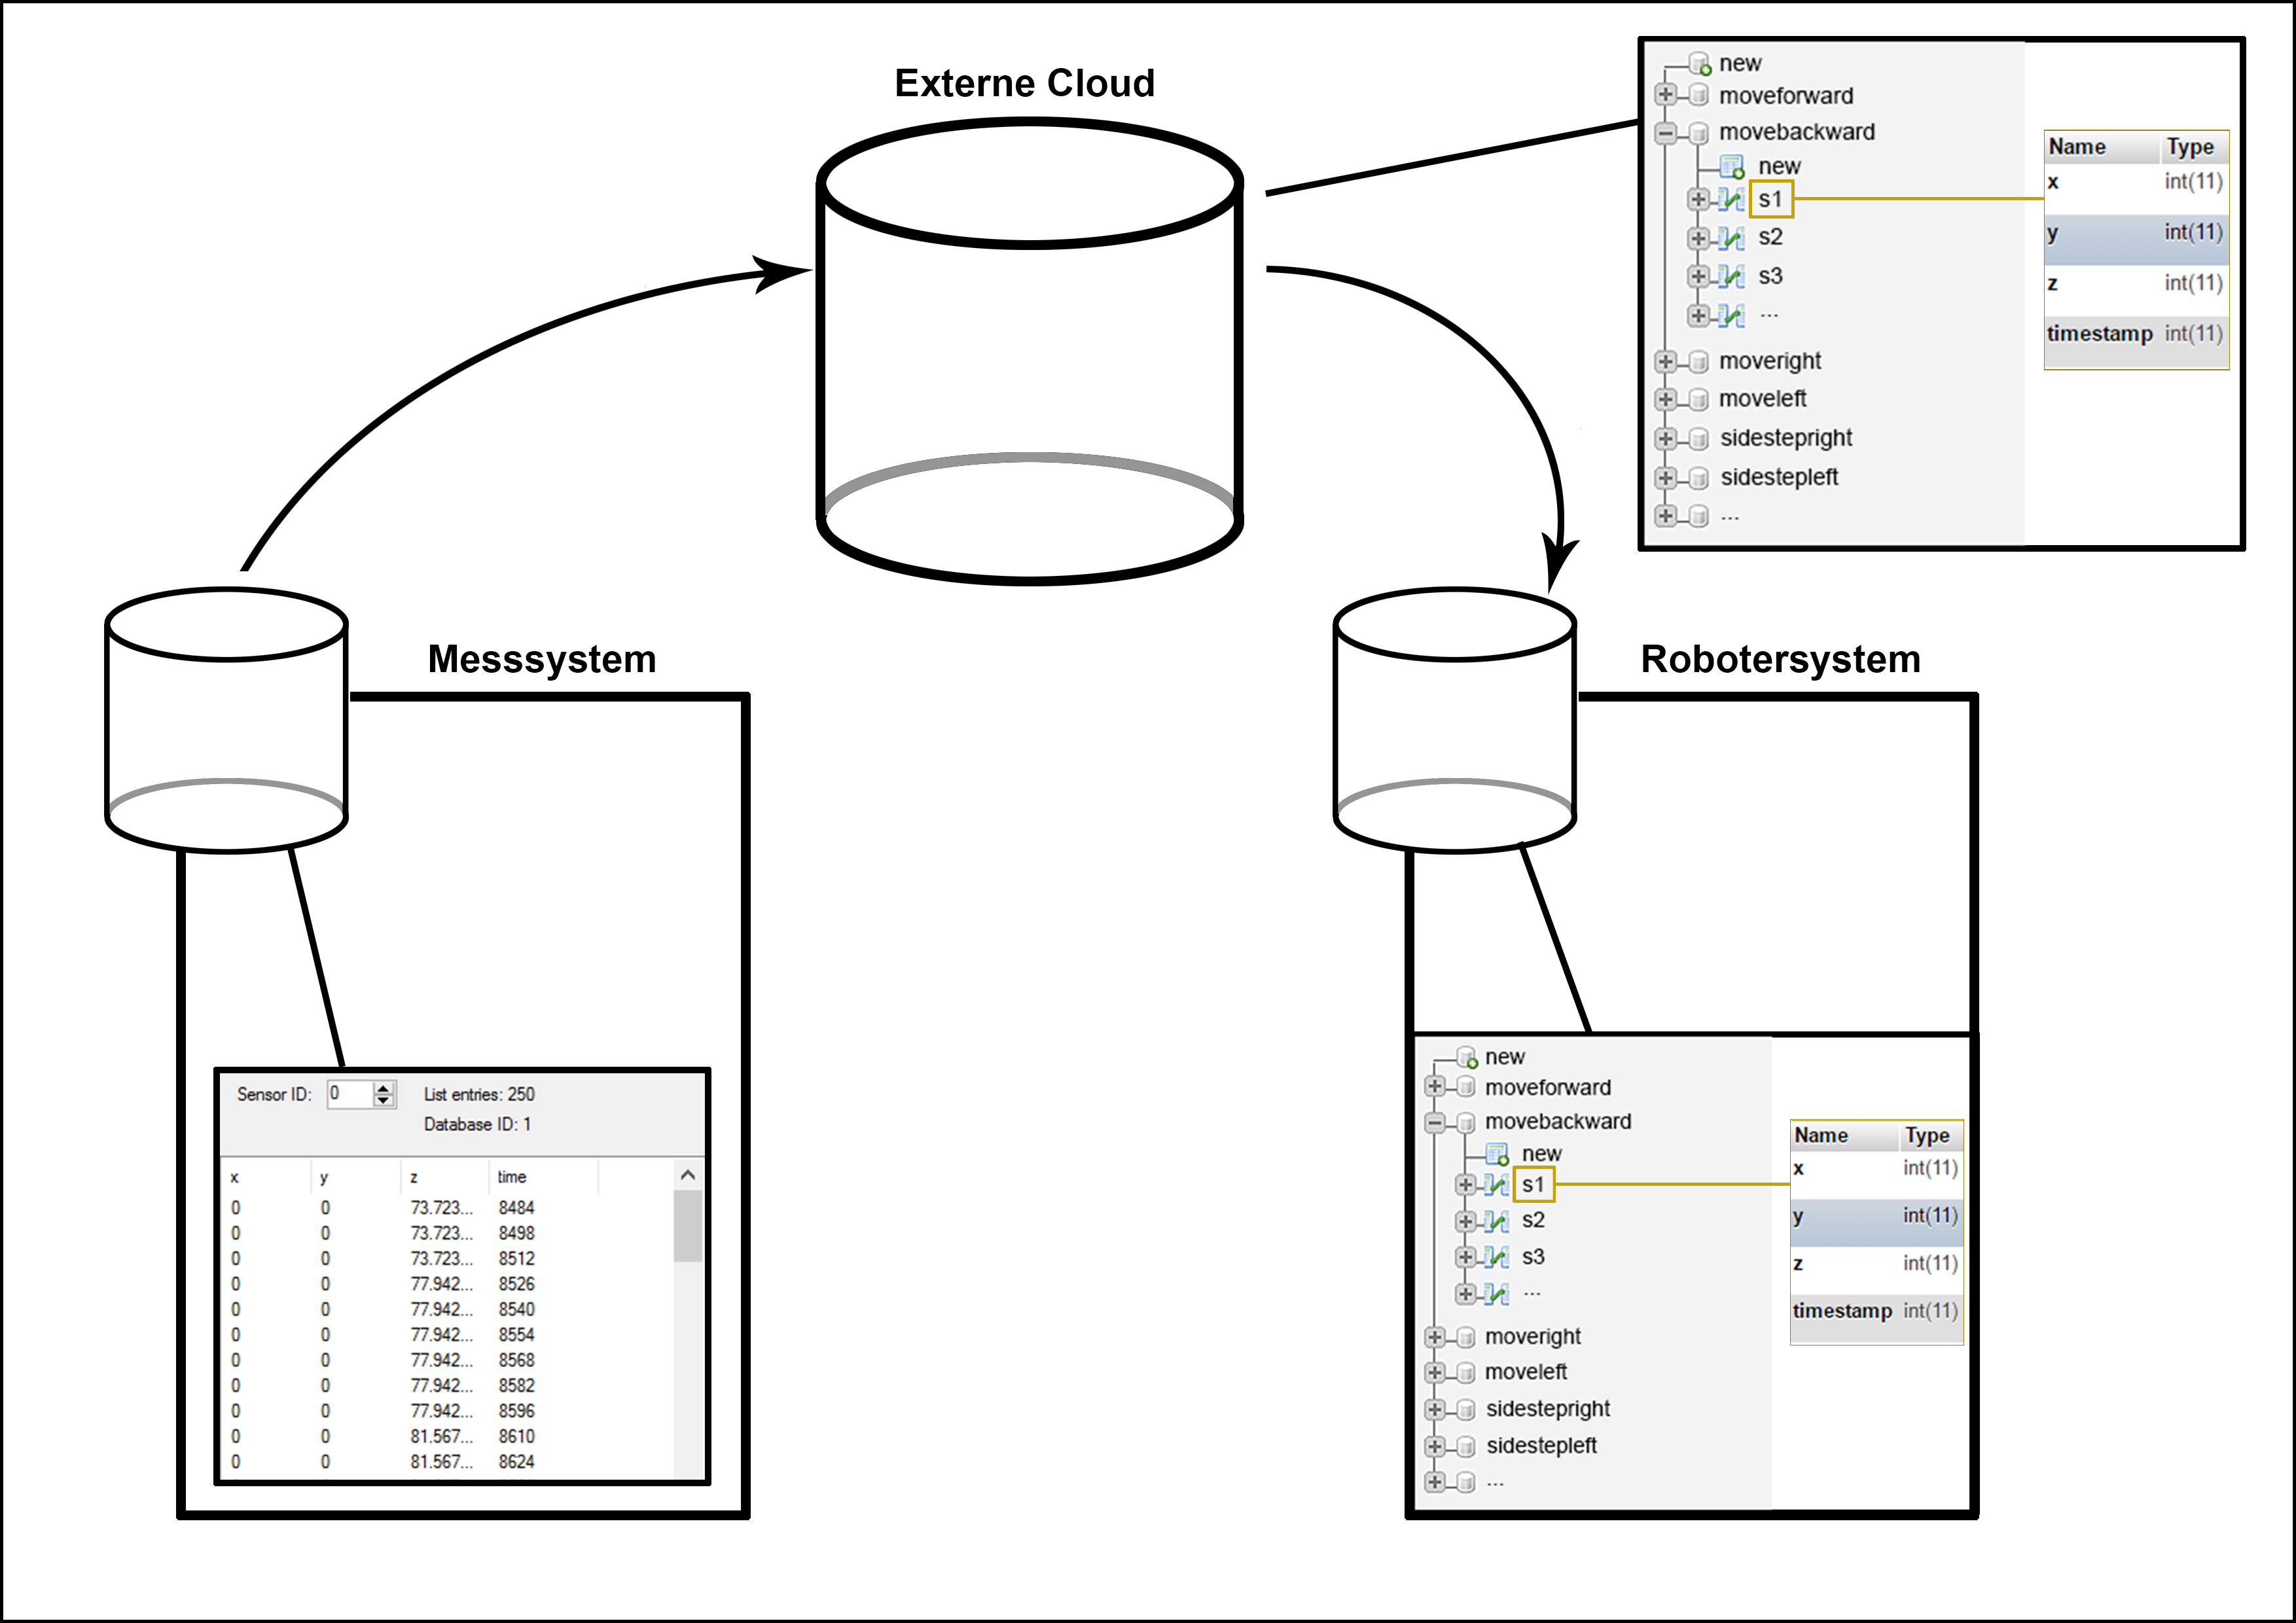
\includegraphics[width=1.0\linewidth]{03_Grafiken/DatabaseLayout/dblayout}
\caption[Layout der Datenbanken]{Layout der Datenbanken}
\label{fig:dblayout}
\end{figure}
